\subsection{Сценарий 2. Simple Reference}

Сценарий Simple Reference сходится, когда агенты правильно перемещаются к своим собственным целевым ориентирам. На \firef{fig-intro-sr} показан скриншот поведения агентов после схождения сценария Simple Reference. В проведённых экспериментах агенты тренировались алгоритмами DDPG и MADDPG.

\begin{figure}[ht!]
    \center
    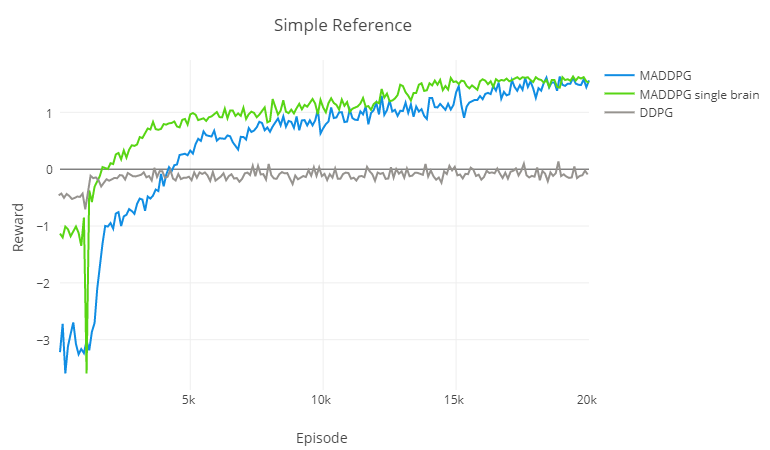
\includegraphics [scale=0.6] {my_folder/images/ch5/sr-rew.png}
    \caption{График среднего вознаграждения для двух агентов в сценарии Simple Reference. Результаты обучения по алгоритму MADDPG, MADDPG с одним мозгом и DDPG}
    \label{fig:result-sr-rew}
\end{figure}

\begin{figure}[ht!]
    \center
    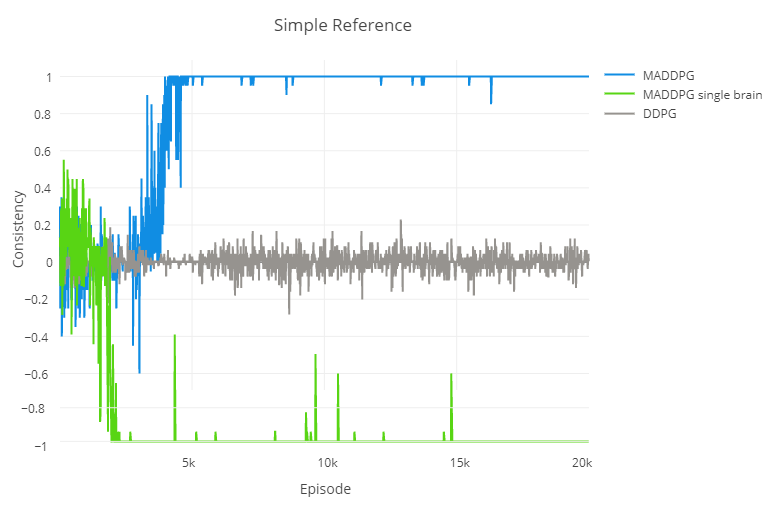
\includegraphics [scale=0.6] {my_folder/images/ch5/sr-comm.png}
    \caption{Графики согласованности взаимодействия для двух агентов в сценарии Simple Reference. Результаты обучения по алгоритму MADDPG, MADDPG с одним мозгом и DDPG}
    \label{fig:result-sr-comm}
\end{figure}

Был построен график вознаграждения для двух агентов, который представлен на \firef{fig:result-sr-rew}. На этом графике синяя кривая~--- результат, обученный MADDPG, зелёная~--- одним мозгом, а серая~--- DDPG.

Агенты, обученные с помощью DDPG, получают меньшее вознаграждение, чем агенты MADDPG и его варианты. Также из рендеринга игры видно, что агенты DDPG блуждают среди ориентиров, не зная, какой из них является правильной целью.

Графики на \firef{fig:result-sr-comm} показывают согласованность действий общения. Для MADDPG и его варианта средний детерминант стремится к 1 или -1. Это указывает на то, что агенты, обученные с помощью этих алгоритмов, могут общаться согласованно. Для агентов, обученных DDPG, значение стремится к 0, это иллюстрируют, что они не могут корректно сообщать цели.

В процессе выполнения многочисленных экспериментов можно было наблюдать, что полная несходимость всегда сопровождается тем, что агенты, не способны дифференцировать и сообщать правильные ориентиры друг другу. То же справедливо и для частичной сходимости, когда агенты могут перемещаться только к тем ориентирам, которые правильно сообщены другими агентами, см. \firef{fig:result-sr-non-convergency}. Это также показывает, что агентам для достижения целей необходимо сотрудничать как в физических, так и в коммуникационных действиях.

\begin{figure}[ht!]
    \center
    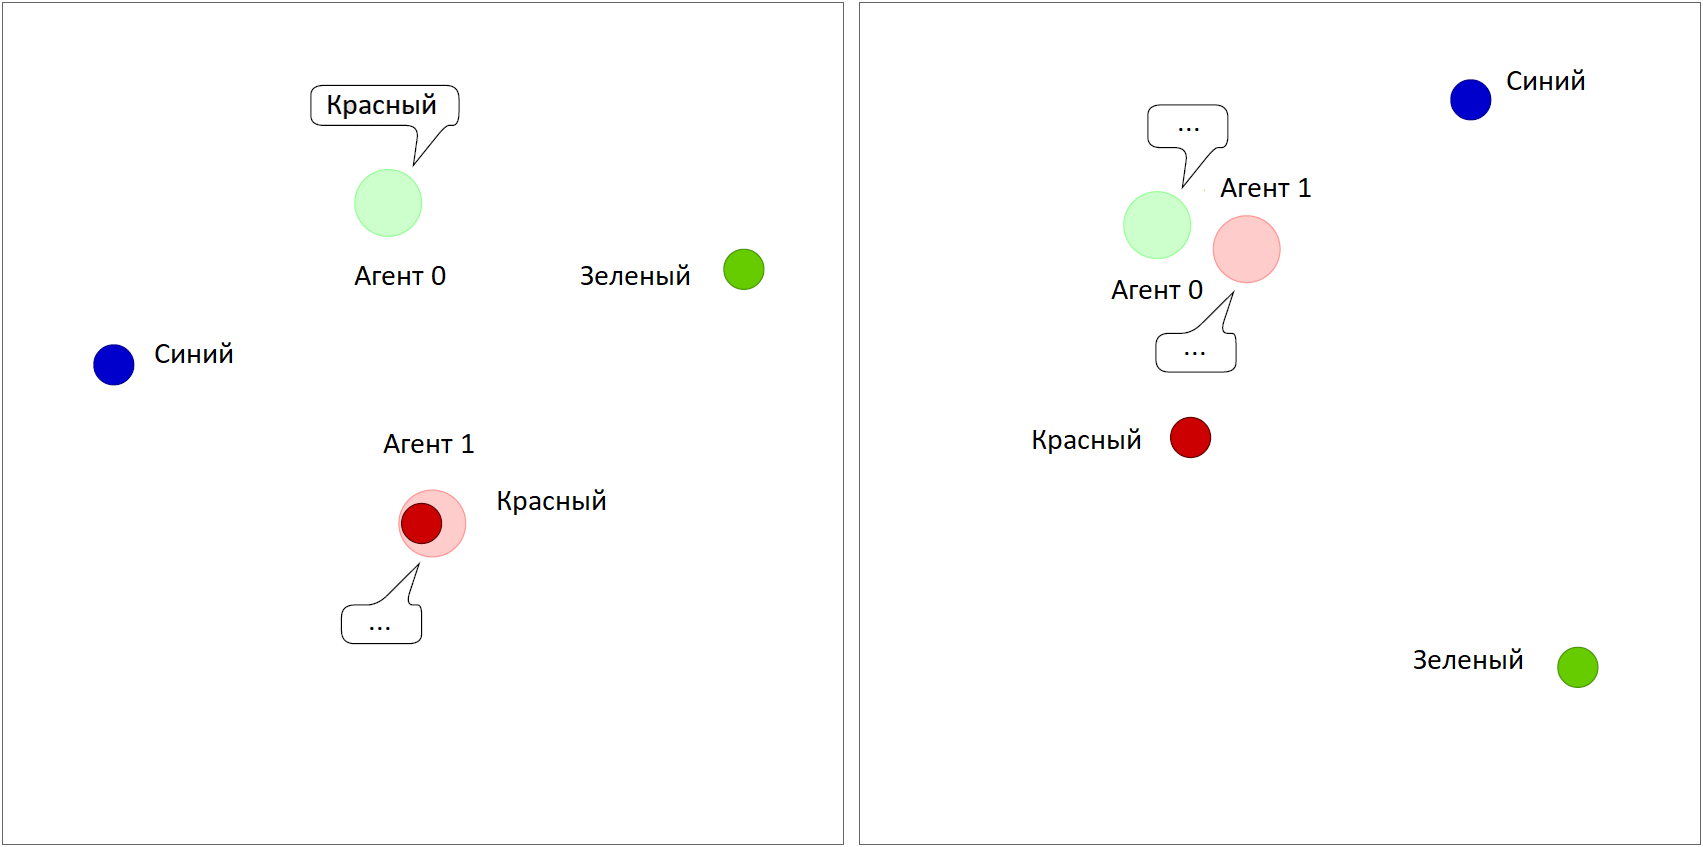
\includegraphics [scale=0.45] {my_folder/images/ch5/results-sr-non-convergency.png}
    \caption{Частичная сходимость с левой стороны: один агент перемещается к цели, а другой ждёт между ориентирами. Несходимость на правой стороне заканчивается тем, что оба агента не знают, куда двигаться и ждут между ориентирами}
    \label{fig:result-sr-non-convergency}
\end{figure}

Наконец, между агентами возникает язык. Проведённые эксперименты показали, что при каждой тренировке агенты по-разному интерпретируют ориентиры. Например, после одной тренировки красный ориентир может выглядеть как ${[1; 0; 0]}$, а после другой~--- как ${[0; 1; 0]}$ или ${[0; 0; 1]}$.

\begin{table}[t!]
    \centering\small
    \caption{Среднее время, потраченное на обучение с различными алгоритмами в 20000 эпизодах}
    \label{tab-sr-time}
    \begin{tabular}{|l|l|l|l|l|l|}
        \hline
        & MADDPG          & MADDPG с одним мозгом \\
        \hline
        Время, 20000 эпизодов & 820 $\pm$ 98~с & 635 $\pm$ 45~с       \\ \hline
    \end{tabular}
    \normalsize% возвращаем шрифт к нормальному
\end{table}

В \taref{tab-sr-time} показано время, затраченное на обучение по сценарию Simple Reference с разными алгоритмами.
